% Created by tikzDevice version 0.12.3.1 on 2021-12-15 13:57:49
% !TEX encoding = UTF-8 Unicode
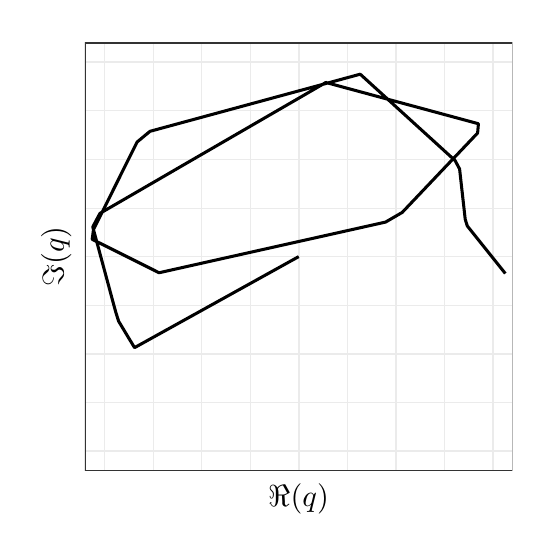
\begin{tikzpicture}[x=1pt,y=1pt]
\definecolor{fillColor}{RGB}{255,255,255}
\path[use as bounding box,fill=fillColor,fill opacity=0.00] (0,0) rectangle (180.67,180.67);
\begin{scope}
\path[clip] (  0.00,  0.00) rectangle (180.67,180.67);
\definecolor{drawColor}{RGB}{255,255,255}
\definecolor{fillColor}{RGB}{255,255,255}

\path[draw=drawColor,line width= 0.6pt,line join=round,line cap=round,fill=fillColor] (  0.00,  0.00) rectangle (180.67,180.68);
\end{scope}
\begin{scope}
\path[clip] ( 20.71, 20.71) rectangle (175.17,175.17);
\definecolor{fillColor}{RGB}{255,255,255}

\path[fill=fillColor] ( 20.71, 20.71) rectangle (175.17,175.17);
\definecolor{drawColor}{gray}{0.92}

\path[draw=drawColor,line width= 0.3pt,line join=round] ( 20.71, 45.29) --
	(175.17, 45.29);

\path[draw=drawColor,line width= 0.3pt,line join=round] ( 20.71, 80.39) --
	(175.17, 80.39);

\path[draw=drawColor,line width= 0.3pt,line join=round] ( 20.71,115.50) --
	(175.17,115.50);

\path[draw=drawColor,line width= 0.3pt,line join=round] ( 20.71,150.60) --
	(175.17,150.60);

\path[draw=drawColor,line width= 0.3pt,line join=round] ( 45.29, 20.71) --
	( 45.29,175.17);

\path[draw=drawColor,line width= 0.3pt,line join=round] ( 80.39, 20.71) --
	( 80.39,175.17);

\path[draw=drawColor,line width= 0.3pt,line join=round] (115.50, 20.71) --
	(115.50,175.17);

\path[draw=drawColor,line width= 0.3pt,line join=round] (150.60, 20.71) --
	(150.60,175.17);

\path[draw=drawColor,line width= 0.6pt,line join=round] ( 20.71, 27.74) --
	(175.17, 27.74);

\path[draw=drawColor,line width= 0.6pt,line join=round] ( 20.71, 62.84) --
	(175.17, 62.84);

\path[draw=drawColor,line width= 0.6pt,line join=round] ( 20.71, 97.94) --
	(175.17, 97.94);

\path[draw=drawColor,line width= 0.6pt,line join=round] ( 20.71,133.05) --
	(175.17,133.05);

\path[draw=drawColor,line width= 0.6pt,line join=round] ( 20.71,168.15) --
	(175.17,168.15);

\path[draw=drawColor,line width= 0.6pt,line join=round] ( 27.74, 20.71) --
	( 27.74,175.17);

\path[draw=drawColor,line width= 0.6pt,line join=round] ( 62.84, 20.71) --
	( 62.84,175.17);

\path[draw=drawColor,line width= 0.6pt,line join=round] ( 97.94, 20.71) --
	( 97.94,175.17);

\path[draw=drawColor,line width= 0.6pt,line join=round] (133.05, 20.71) --
	(133.05,175.17);

\path[draw=drawColor,line width= 0.6pt,line join=round] (168.15, 20.71) --
	(168.15,175.17);
\definecolor{drawColor}{RGB}{0,0,0}

\path[draw=drawColor,line width= 1.1pt,line join=round] (172.60, 91.84) --
	(170.88, 93.98) --
	(169.17, 96.13) --
	(167.45, 98.27) --
	(165.73,100.42) --
	(164.01,102.56) --
	(162.30,104.71) --
	(160.58,106.85) --
	(158.86,109.00) --
	(158.10,111.44) --
	(157.81,114.04) --
	(157.52,116.64) --
	(157.23,119.23) --
	(156.94,121.83) --
	(156.65,124.42) --
	(156.36,127.02) --
	(156.07,129.61) --
	(154.45,132.64) --
	(150.17,136.54) --
	(145.88,140.45) --
	(141.59,144.35) --
	(137.31,148.25) --
	(133.02,152.15) --
	(128.74,156.06) --
	(124.45,159.96) --
	(120.17,163.86) --
	(110.67,161.28) --
	(101.18,158.70) --
	( 91.68,156.12) --
	( 82.19,153.54) --
	( 72.69,150.96) --
	( 63.20,148.38) --
	( 53.70,145.80) --
	( 44.21,143.22) --
	( 39.54,139.35) --
	( 37.29,134.83) --
	( 35.04,130.31) --
	( 32.79,125.80) --
	( 30.54,121.28) --
	( 28.29,116.76) --
	( 26.04,112.24) --
	( 23.79,107.72) --
	( 23.30,104.20) --
	( 26.33,102.69) --
	( 29.35,101.18) --
	( 32.37, 99.67) --
	( 35.39, 98.16) --
	( 38.41, 96.65) --
	( 41.44, 95.14) --
	( 44.46, 93.63) --
	( 47.48, 92.11) --
	( 57.71, 94.40) --
	( 67.94, 96.69) --
	( 78.18, 98.98) --
	( 88.41,101.27) --
	( 98.64,103.56) --
	(108.87,105.84) --
	(119.10,108.13) --
	(129.33,110.42) --
	(135.34,113.91) --
	(139.23,118.01) --
	(143.12,122.11) --
	(147.01,126.21) --
	(150.90,130.31) --
	(154.80,134.40) --
	(158.69,138.50) --
	(162.58,142.60) --
	(162.88,145.95) --
	(155.99,147.82) --
	(149.10,149.68) --
	(142.21,151.55) --
	(135.31,153.41) --
	(128.42,155.27) --
	(121.53,157.14) --
	(114.64,159.00) --
	(107.75,160.87) --
	( 97.55,154.95) --
	( 87.34,149.04) --
	( 77.14,143.13) --
	( 66.94,137.22) --
	( 56.73,131.31) --
	( 46.53,125.39) --
	( 36.33,119.48) --
	( 26.12,113.57) --
	( 23.51,108.67) --
	( 24.70,104.29) --
	( 25.88, 99.90) --
	( 27.06, 95.52) --
	( 28.25, 91.13) --
	( 29.43, 86.75) --
	( 30.61, 82.36) --
	( 31.80, 77.98) --
	( 32.86, 74.60) --
	( 33.68, 73.24) --
	( 34.50, 71.87) --
	( 35.32, 70.50) --
	( 36.14, 69.14) --
	( 36.97, 67.77) --
	( 37.79, 66.41) --
	( 38.61, 65.04) --
	( 97.94, 97.94);
\definecolor{drawColor}{gray}{0.20}

\path[draw=drawColor,line width= 0.6pt,line join=round,line cap=round] ( 20.71, 20.71) rectangle (175.17,175.17);
\end{scope}
\begin{scope}
\path[clip] (  0.00,  0.00) rectangle (180.67,180.67);
\definecolor{drawColor}{RGB}{0,0,0}

\node[text=drawColor,anchor=base,inner sep=0pt, outer sep=0pt, scale=  1.10] at ( 97.94,  7.64) {$\Re(q)$};
\end{scope}
\begin{scope}
\path[clip] (  0.00,  0.00) rectangle (180.67,180.67);
\definecolor{drawColor}{RGB}{0,0,0}

\node[text=drawColor,rotate= 90.00,anchor=base,inner sep=0pt, outer sep=0pt, scale=  1.10] at ( 13.08, 97.94) {$\Im(q)$};
\end{scope}
\end{tikzpicture}
